%\documentclass[dvipdfmx]{beamer}      % platex の場合
\documentclass{beamer}                 % lualatex の場合
\usepackage{mySld}
\usepackage{multicol}

\begin{document}
\title{基礎コンピュータ工学\\第5章 機械語プログラミング\\(パート3)}
\date{}

\begin{frame}
  \titlepage
  \centerline{\url{https://github.com/tctsigemura/TecTextBook}}
  \vfill
  \centerline{本スライドの入手:
    \raisebox{-7mm}{
\includegraphics[scale=0.3]{../Img/QRs5_3.png}}}
\end{frame}

%==============================================================================
%\begin{frame}
%  \frametitle
%  \tableofcontents
%\end{frame}

\section{算術演算命令}
%==============================================================================
\begin{frame}
  \frametitle{算術演算命令(2種類)}
  算術計算(普通の計算)をする命令
  \begin{itemize}
  \item \texttt{ADD(Add)命令}: 加算命令(足し算をする) \\
    CPUのレジスタ ← CPUのレジスタ \texttt{+} メモリ
  \item \texttt{SUB(Subtract)命令}: 減算命令(引き算をする) \\
    CPUのレジスタ ← CPUのレジスタ \texttt{-} メモリ
  \end{itemize}
  \vfill
  CPUのレジスタは一つだけ使用できる.\\
  \begin{itemize}
  \item \texttt{ADD命令}の例:\\
    \texttt{G0 ← G0 + [EA]}
  \item \texttt{SUB命令}の例:\\
    \texttt{G1 ← G1 - [EA]}
  \end{itemize}
\end{frame}

%==============================================================================
\begin{frame}
  \frametitle{ADD(Add)命令(ニーモニックと命令フォーマット)}
  メモリ(\texttt{EA})のデータをCPUのレジスタ(\texttt{GR})足し込む.

  \begin{description}
  \item[ニーモニック:]\texttt{ADD GR,EA}~~~~~~~~~\texttt{(GR ← GR + [EA])}
    \vfill

  \item[命令フォーマット:] 2バイトの長さを持つ.\\
    \twoByte{$0011_2$}{\GR~\XR}{\A}
  \end{description}
  \vfill

  \emph{例:}メモリの3番地のデータをG2レジスタへ足し込む.
  \begin{description}
  \item[ニーモニック:]\texttt{ADD G2,03H}~~~~~~~~~動作:

  \item[命令フォーマット:] G2と03Hを反映する.\\
    \twoByte{$0011_2$}{$10_2$~$00_2$}{$0000~0011_2$}
  \end{description}
  \vfill
\end{frame}

%==============================================================================
\begin{frame}
  \frametitle{ADD(Add)命令(フローチャートの描き方)}
  \begin{description}
  \item[ADD命令のフローチャート:] \texttt{[}と\texttt{]}を忘れないように!\\
    \centerline{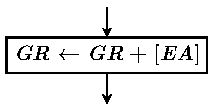
\includegraphics[scale=0.8]{../Tikz/add.pdf}}
    \vfill
    
  \item[例:]7番地のデータと8番地のデータの和を9番地に求める.\\
    (今回はG0を使用してみた.)\\
    \centerline{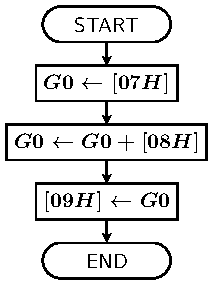
\includegraphics[scale=0.8]{../Tikz/adds.pdf}}
    \vfill
  \end{description}
\end{frame}

%==============================================================================
\begin{frame}
  \frametitle{ADD(Add)命令(プログラム例)}
  \begin{description}
  \item[プログラムの例:]7番地と8番地のデータの和を9番地に求める.\\
    {\ttfamily\small\begin{center}
      \begin{tabular}{|l|l|l|l l|} \hline
        番地 & 機械語 & ラベル & \multicolumn{2}{|c|}{ニーモニック} \\
        \hline
        00 & 10 07 & & LD   & G0,07H \\
        02 & 30 08 & & ADD  & G0,08H \\
        04 & 20 09 & & ST   & G0,09H \\
        06 & FF    & & HALT & \\
        \hline
      \end{tabular}
    \end{center}}
    \vfill

    \item[メモリに格納した状態:] 何かデータも準備する必要がある.
      {\ttfamily\small\begin{center}
        \begin{tabular}{r|c|l}
          \multicolumn{1}{c}{番地} &
          \multicolumn{1}{c}{機械語} &
          \multicolumn{1}{c}{意味} \\
          \cline{2-2}
          $00$ & $10$ & LD G0,07H \\
          \cline{2-2}
          $01$ & $07$ &           \\
          \cline{2-2}
          $02$ & $30$ & ADD G0,08H \\
          \cline{2-2}
          $03$ & $08$ &           \\
          \cline{2-2}
          $04$ & $20$ & ST G0,09H \\
          \cline{2-2}
          $05$ & $09$ &           \\
          \cline{2-2}
          $06$ & $FF$ & HALT      \\
          \cline{2-2}
          $07$ & $12$ & データ!!\\
          \cline{2-2}
          $08$ & $34$ & データ!!\\
          \cline{2-2}
          $09$ & $00$ & データ!!\\
          \cline{2-2}
        \end{tabular}
      \end{center}}
      \vfill

  \end{description}
\end{frame}

%==============================================================================
\begin{frame}
  \frametitle{SUB(Subtract)命令(ニーモニックとフォーマット)}
  メモリ(\texttt{EA})のデータをCPUのレジスタ(\texttt{GR})から引く.

  \begin{description}
  \item[ニーモニック:]\texttt{SUB GR,EA}~~~~~~~~~\texttt{(GR ← GR - [EA])}
    \vfill

  \item[命令フォーマット:] 2バイトの長さを持つ.\\
    \twoByte{$0100_2$}{\GR~\XR}{\A}
  \end{description}
  \vfill

  \emph{例:}メモリの3番地のデータをG1レジスタから引く.
  \begin{description}
  \item[ニーモニック:]\texttt{SUB G1,03H}~~~~~~~~~動作:

  \item[命令フォーマット:] G1と03Hを反映する.\\
    \twoByte{$0100_2$}{$01_2$~$00_2$}{$0000~0011_2$}
  \end{description}
  \vfill
\end{frame}

%==============================================================================
\begin{frame}
  \frametitle{SUB(Subtract)命令(フローチャートの描き方)}
  \begin{description}
  \item[SUB命令のフローチャート:] \texttt{[}と\texttt{]}を忘れないように!\\
    \centerline{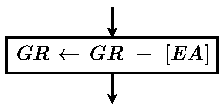
\includegraphics[scale=0.8]{../Tikz/sub.pdf}}
    \vfill
    
  \item[例:]7番地のデータと8番地のデータの\emph{差}を9番地に求める.\\
    (今回はG1を使用してみた.)\\
    \centerline{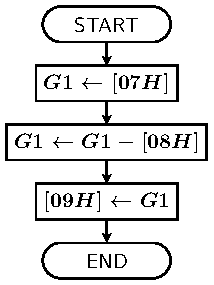
\includegraphics[scale=0.8]{../Tikz/subs.pdf}}
    \vfill
  \end{description}
\end{frame}

%==============================================================================
\begin{frame}
  \frametitle{SUB(Subtract)命令(プログラム例)}
  \begin{description}
  \item[プログラムの例:]7番地と8番地のデータの\emph{差}を9番地に求める.\\
    {\ttfamily\small\begin{center}
      \begin{tabular}{|l|l|l|l l|} \hline
        番地 & 機械語 & ラベル & \multicolumn{2}{|c|}{ニーモニック} \\
        \hline
        00 & 14 07 & & LD   & G1,07H \\
        02 & 44 08 & & SUB  & G1,08H \\
        04 & 24 09 & & ST   & G1,09H \\
        06 & FF    & & HALT & \\
        \hline
      \end{tabular}
    \end{center}}
    \vfill

    \item[メモリに格納した状態:] 何かデータも準備する必要がある.
      {\ttfamily\small\begin{center}
        \begin{tabular}{r|c|l}
          \multicolumn{1}{c}{番地} &
          \multicolumn{1}{c}{機械語} &
          \multicolumn{1}{c}{意味} \\
          \cline{2-2}
          $00$ & $14$ & LD G1,07H \\
          \cline{2-2}
          $01$ & $07$ &           \\
          \cline{2-2}
          $02$ & $44$ & SUB G1,08H \\
          \cline{2-2}
          $03$ & $08$ &           \\
          \cline{2-2}
          $04$ & $24$ & ST G1,09H \\
          \cline{2-2}
          $05$ & $09$ &           \\
          \cline{2-2}
          $06$ & $FF$ & HALT      \\
          \cline{2-2}
          $07$ & $0A$ & データ!!\\
          \cline{2-2}
          $08$ & $03$ & データ!!\\
          \cline{2-2}
          $09$ & $00$ & データ!!\\
          \cline{2-2}
        \end{tabular}
      \end{center}}
      \vfill

  \end{description}
\end{frame}

%==============================================================================
%\newcommand{\kai}[1]{{\color{red}{#1}\color{black}}}
\newcommand{\kai}[1]{{\color{white}{#1}\color{black}}}
\begin{frame}
  \frametitle{演習(1)}
  足し算プログラム,引き算プログラムのデータを変更して計算結果を確認しなさい.
  \vfill
  
  \begin{tabular}{c c c}
    \begin{minipage}{0.3\columnwidth}
      {\ttfamily\small\begin{tabular}{ l l l }
        & 0000 1010   & (10) \\
        + & 0000 1010 & (10) \\
        \cline{1-2}
        & 0001 0100   & (20) \\
      \end{tabular}}
    \end{minipage}
    &
    \begin{minipage}{0.3\columnwidth}
      {\ttfamily\small\begin{tabular}{ l l l }
        & 0000 1010   & ( 10) \\
        + & 1111 0110 & (-10) \\
        \cline{1-2}
        & \kai{0000 0000} & (\kai{~~0})\\
      \end{tabular}}
    \end{minipage}
    &
    \begin{minipage}{0.3\columnwidth}
      {\ttfamily\small\begin{tabular}{ l l l }
        & 1100 0000   & (-64)\\
        + & 0111 0000 & (112)\\
        \cline{1-2}
        & \kai{0011 0000} & (\kai{ 48})\\
      \end{tabular}}
    \end{minipage}
    \\
    &&\\
    &&\\
    \begin{minipage}{0.3\columnwidth}
      {\ttfamily\small\begin{tabular}{ l l l }
        & 0000 1010   & (\kai{10})\\
        - & 0000 0101 & (\kai{ 5})\\
        \cline{1-2}
        & \kai{0000 0101} & (\kai{ 5})\\
      \end{tabular}}
    \end{minipage}
    &
    \begin{minipage}{0.3\columnwidth}
      {\ttfamily\small\begin{tabular}{ l l l }
        & 0000 1100   & ( 12)\\
        - & 1111 0011 & (-13)\\
        \cline{1-2}
        & \kai{0001 1001} & (\kai{ 25})\\
      \end{tabular}}
    \end{minipage}
    &
    \begin{minipage}{0.3\columnwidth}
      {\ttfamily\small\begin{tabular}{ l l l }
        & 0000 0000   & ( 0) \\
        - & 0000 0001 & ( 1) \\
        \cline{1-2}
        & \kai{1111 1111} & (\kai{-1}) \\
      \end{tabular}}
    \end{minipage}
    \\
  \end{tabular}
  \vfill
  
\end{frame}

%==============================================================================
\begin{frame}
  \frametitle{演習(2)}
  次の手順を守って演習を行う.
  \begin{enumerate}
  \item[1.] フローチャートを描いて考えをまとめる.
  \item[2.] ニーモニック(オペレーション,オペランド)に変換する.
  \item[3.] 番地(アドレス)を決める.
  \item[4.] 機械語を決める.
  \item[5.] TeCに打ち込み実行して結果を確認する.
  \end{enumerate}
  \centerline{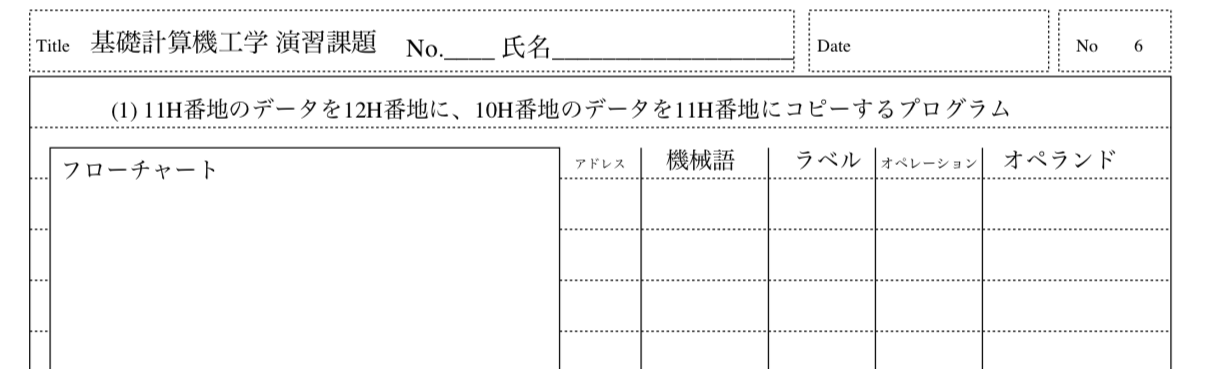
\includegraphics[scale=0.5]{tejyun.png}}
  \vfill
  \vfill
\end{frame}

%==============================================================================
%\begin{frame}
%  \frametitle{}
%\end{frame}

\end{document}
